\section{Static Model \& Inference}
\label{sec:static}

%We review interferometric imaging for a static emission in the case of a multivariate Gaussian image prior. The techniques and insights obtained in this section will lead to 


Before discussing our proposed approach to dynamic imaging for time-varying sources, we first review %the basics of 
interferometric imaging for a static source and discuss a simple, yet instructive, approach using a multivariate Gaussian image prior. 
The intent of this section is {\it not} to present a novel and competitive static imaging method, but instead to set up the tools necessary to easily understand dynamic imaging in Sections~\ref{sec:dynamic_model} and~\ref{sec:dynamic_inference}.
%For simplicity, in this section we assume measurements are a vector of complex visibilities, $y$, with Gaussian noise (i.e. no atmospheric error), of variance $\sigma^2$. 

We measure 
a vector of real values $\meas$ 
%(e.g $y = [\Re (\bm{\vis}), \Im( \bm{\vis})]^T$), 
that are generated by observing a static source's emission region image, $I(\xpos, \ypos)$. These measurements are extremely sparse and noisy, and thus do not fully characterize the underlying image. 
For example, a simple PCA analysis on rows of the DTFT matrix $\FTmtx$ for the EHT 2017 campaign (see the uv-coverage of Fig.~\ref{fig:staticimaging}) shows that 95\% of the variance can be described using only 1624 measurement sub-functions, $g(\im)$, for a 10000 pixel image; essentially $\FTmtx$ constrains only 16\% of the unknowns. 
To solve this problem, we impose a prior distribution on $\im$ and seek a maximum a posteriori (MAP) estimate of the underlying image given these sparse observations. We adopt the model presented in~\cite{bouman2016computational} to represent $I(\xpos, \ypos)$ as vectorized coefficients, $\im$. Using this representation, we define our observation model as:
\begin{align}
\meas & \sim \mathcal{N}_{\meas}(f(\im), \bR), \\
\im & \sim \mathcal{N}_{\im}(\bmu, \bLambda),
\end{align}
\noindent{where $\mathcal{N}_{z}(m, \Sigma)$ is the multivariate normal distribution of $z$ with mean $m$ and covariance $\Sigma$. In the chosen model, both the data likelihood, $p(\meas|\im)$, and the underlying image prior, $p(\im)$, are multivariate normal distributions. The posterior probability is written in terms of these two terms: % the data likelihood, $p(\meas|\im)$, and the image prior, $p(\im)$. 
}
\begin{align} 
\label{eq:bayes}
p(\im|\meas) & \propto p(\meas|\im) p(\im) \\
\notag & = \mathcal{N}_{\meas}(f(\im), \bR) \mathcal{N}_{\im}(\bmu, \bLambda).
\end{align}

%In this model we assume that both the observed data products, $\meas$, and the true underlying image, $\im$, are samples from multivariate Gaussian distributions. 
%Note that Equation BLAH is only valid if every linear combination of $\meas$ results in a univariate Gaussian distribution. 
Unfortunately, $p(\meas|\im)$ is not truly Gaussian when $\meas$ is composed of bispectra or closure phases, as each visibility is used to compute multiple terms. However, as discussed in Section~\ref{sec:bispec}, we assume that each term of $\meas$ is independent and can be described with a Gaussian noise model. This approximation has been shown to be a good approximation in practice (see the supplemental material)~\cite{TMS,bouman2016computational}.

%Each vector of measured data products, $\meas$, is assumed to be a function of an underlying image, $\im$, (refer to Section BLAH) with added Gaussian noise. The true underlying image, $\im$, is assumed to be a sample from a multivariate Gaussian distribution. 

\begin{figure}[tb]
                       	\begin{center}
                       		\begin{tabular}{  c | c | c   }
                       			%\hline
                       			&\large{\textsf{$\bLambda$}}   &\large{\textsf{SAMPLES }} \hspace{.55in}   \\ \hline
                     
&\vspace{-.1in}& \\
                       			\multirow{1}{*}[.6in]{ \rotatebox[origin=t]{90}{\large{\textsf{a = 2}} }}
                                &
{{ 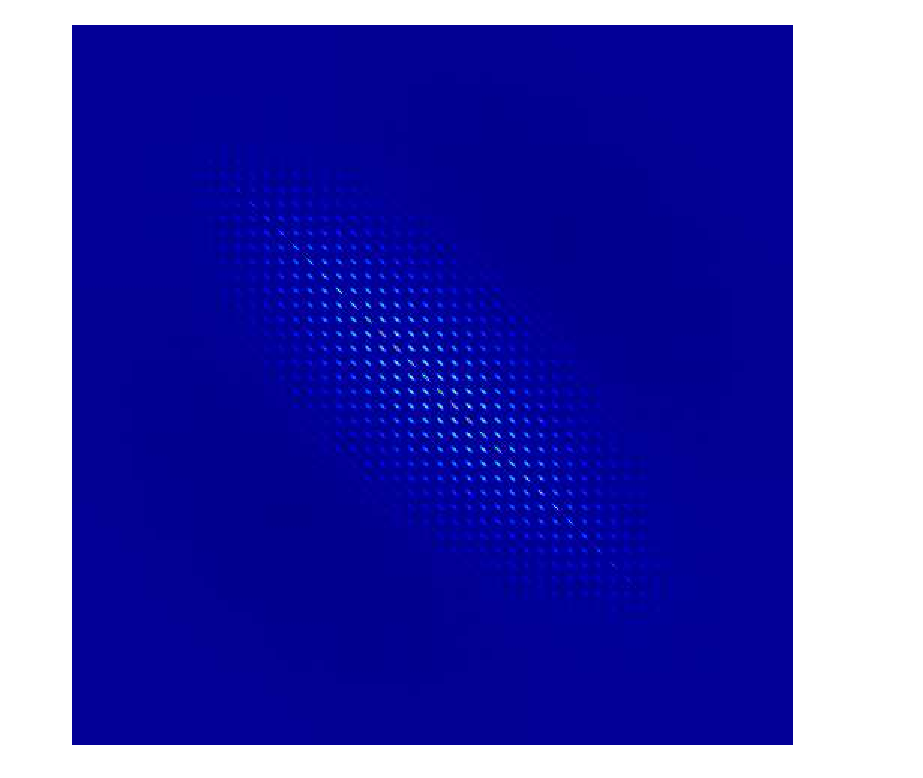
\includegraphics[width=0.2\linewidth]{figures/prior/outfile_drop2_cropped.pdf}} } &
                       			{ 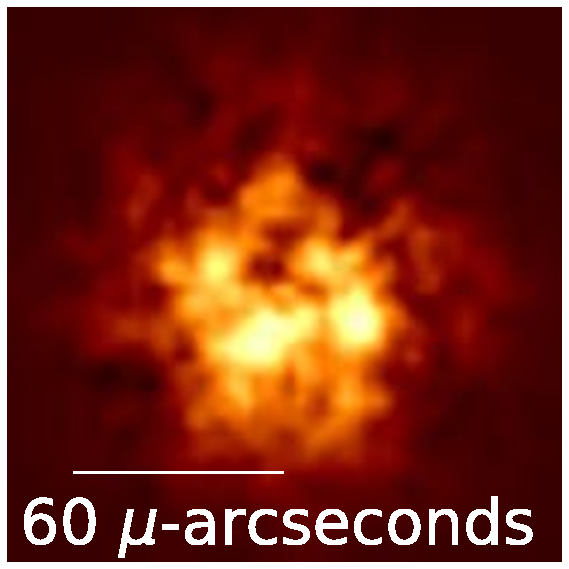
\includegraphics[width=0.2\linewidth]{figures/prior/newfiles/sampfig_drop2_1_scale2.pdf}} 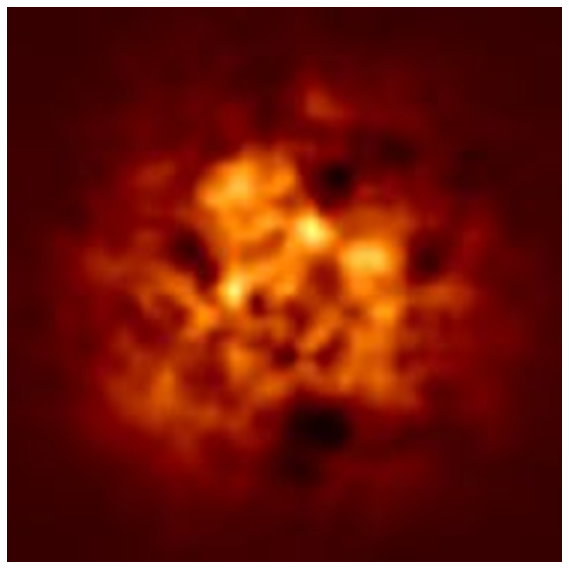
\includegraphics[width=0.2\linewidth]{figures/prior/newfiles/sampfig_drop2_4.pdf} 
                       			\multirow{3}{*}[.6in]{ 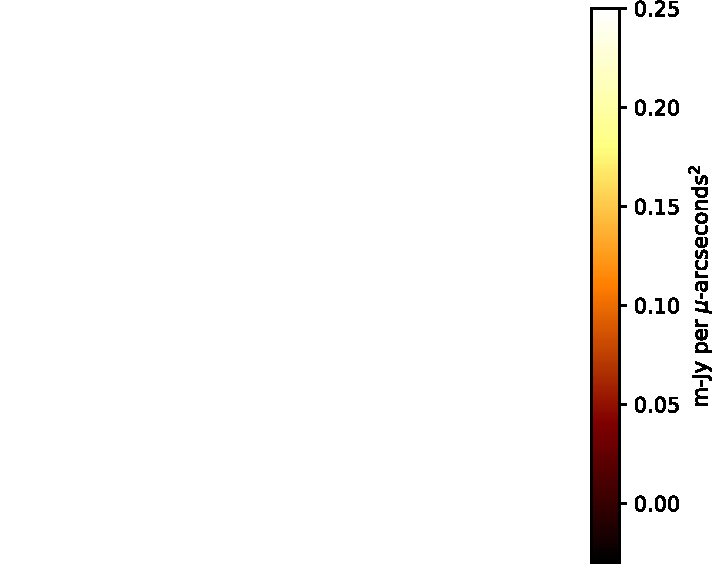
\includegraphics[width=0.155\linewidth]{figures/prior/newfiles/sampfig_drop2_1_cbar.pdf} }
                                \\
                       			&\vspace{-.1in}&\\
                       			\multirow{1}{*}[.6in]{ \rotatebox[origin=t]{90}{\large{\textsf{a = 3}} }} & 
                       			{{ 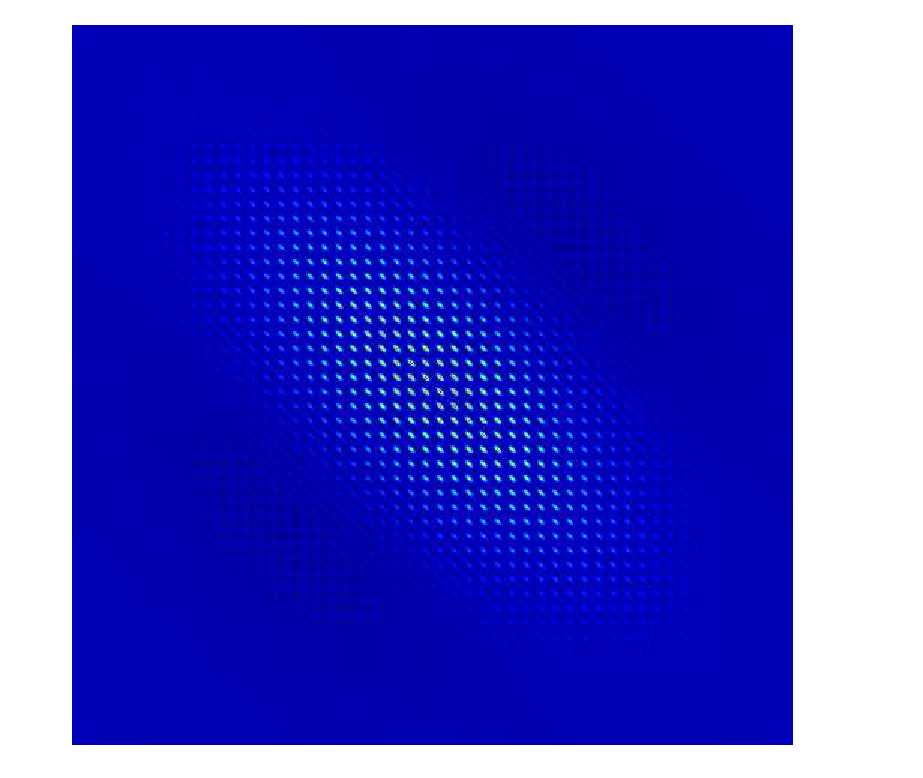
\includegraphics[height=0.2\linewidth]{figures/prior/outfile_drop3_cropped.pdf}} } &
                       			{ 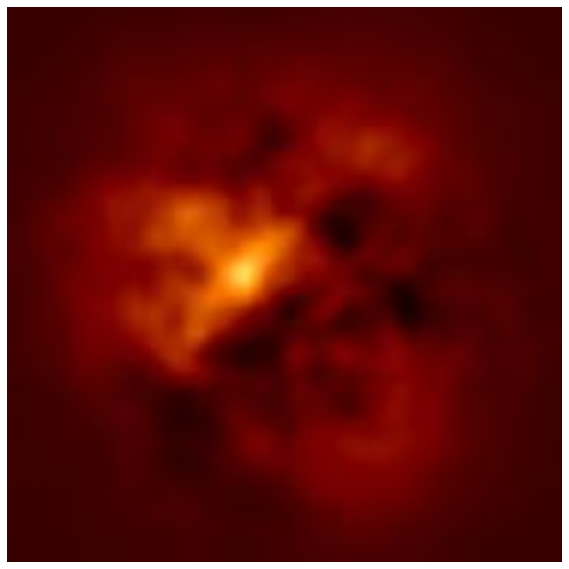
\includegraphics[height=0.2\linewidth]{figures/prior/newfiles/sampfig_drop3_2.pdf}} 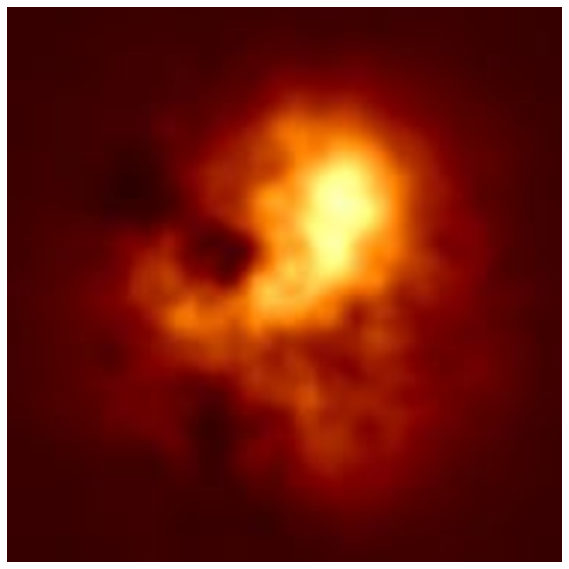
\includegraphics[height=0.2\linewidth]{figures/prior/newfiles/sampfig_drop3_3.pdf}  
                       			\hspace{.65in}
                       			%\multirow{3}{*}[.6in]{ 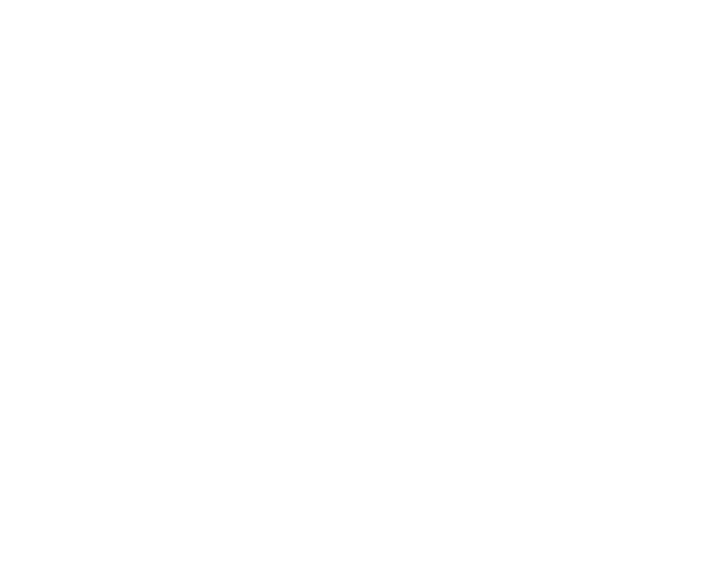
\includegraphics[width=0.18\linewidth]{figures/prior/newfiles/placeholder.pdf} }
                       			\\
                       			&\vspace{-.1in}& \\
                       			\multirow{1}{*}[.6in]{ \rotatebox[origin=t]{90}{\large{\textsf{a = 4}} }} & 
                       			{{ 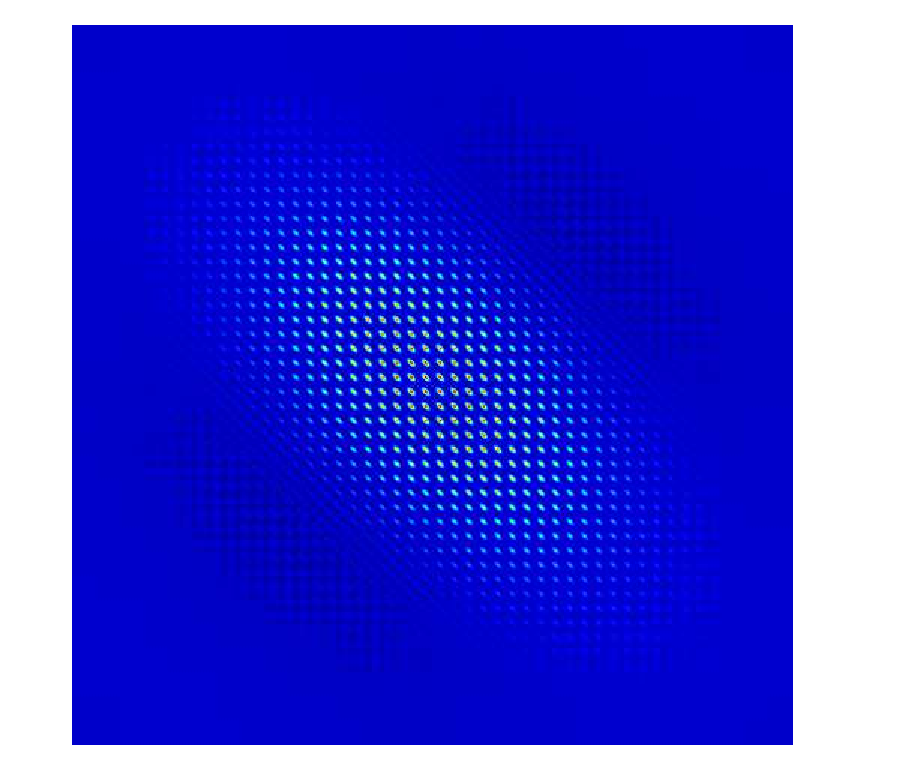
\includegraphics[height=0.2\linewidth]{figures/prior/outfile_drop4_cropped.pdf}} } &
                       			{ 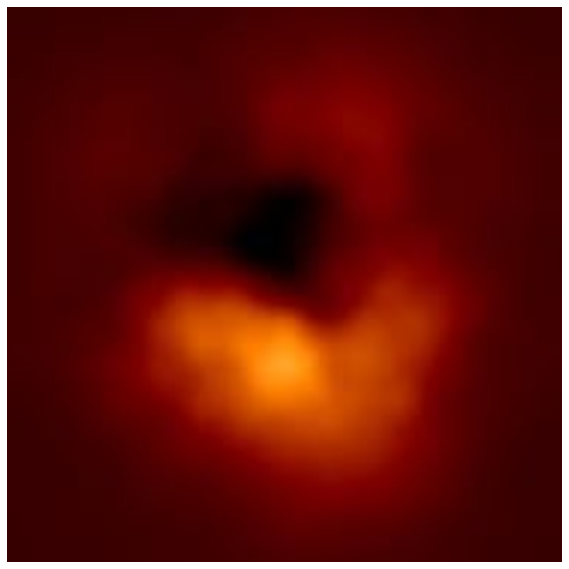
\includegraphics[height=0.2\linewidth]{figures/prior/newfiles/sampfig_drop4_1.pdf}} 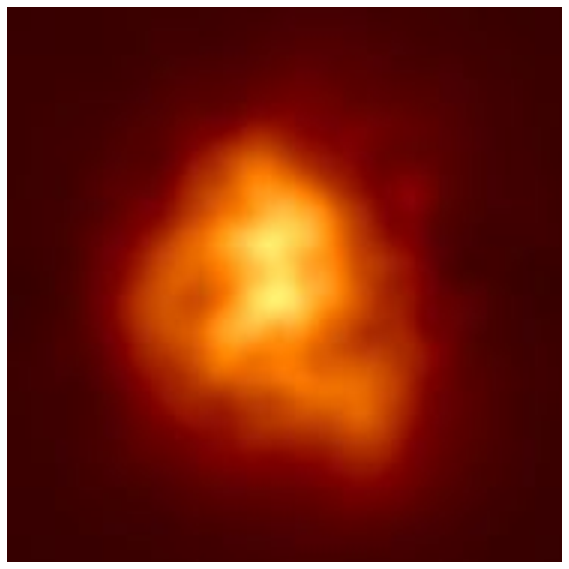
\includegraphics[height=0.2\linewidth]{figures/prior/newfiles/sampfig_drop4_2.pdf}                        			
                       			\hspace{.65in}
                       			%\multirow{3}{*}[.6in]{ 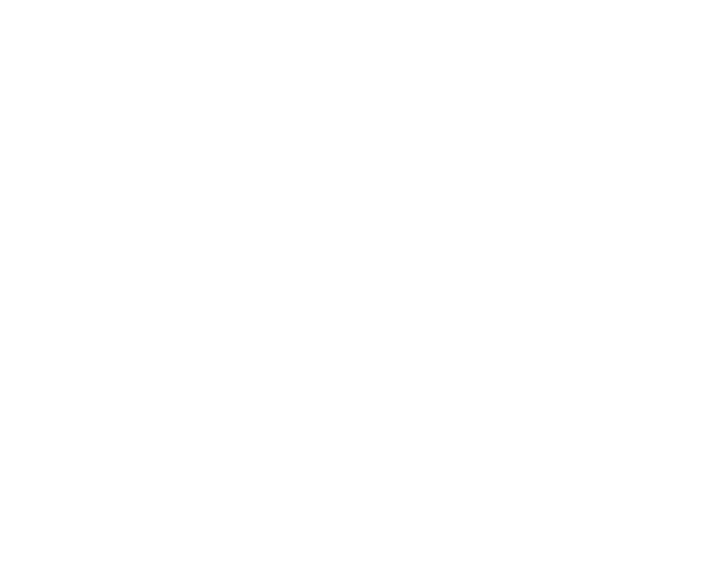
\includegraphics[width=0.18\linewidth]{figures/prior/newfiles/placeholder.pdf} } 
                       			\\            	
                       		\end{tabular}
                       		\caption{\footnotesize{{\bf Gaussian Image Prior:} The covariance matrix constructed for $a=2,3,4$ along with image samples from the prior  $\mathcal{N}_x(\mu, \Lambda)$. The image samples have a field of view of 160 $\mu$-arcseconds. Notice that as $a$ increases, the sampled images appear smoother (i.e., the prior encourages smoother structure). In these examples $\mu$ is a 2D Gaussian image with standard deviation of 75 $\mu$-arcseconds. and $c=0.5$. 
                       			}}
                       			\label{fig:priorsamples}
\end{center}
\vspace{-.2in}
\end{figure}

\begin{figure*}[h!]
	\vspace{-.0in}
	\setlength{\tabcolsep}{1pt}
	\begin{center}
		\begin{tabular}{ c  c  | c  c  c c  }
			%\hline
			 \hspace*{-1.0cm}  
             \multirow{4}{*}[-0in]{ \rotatebox[origin=t]{0}{ {\vspace*{1in} 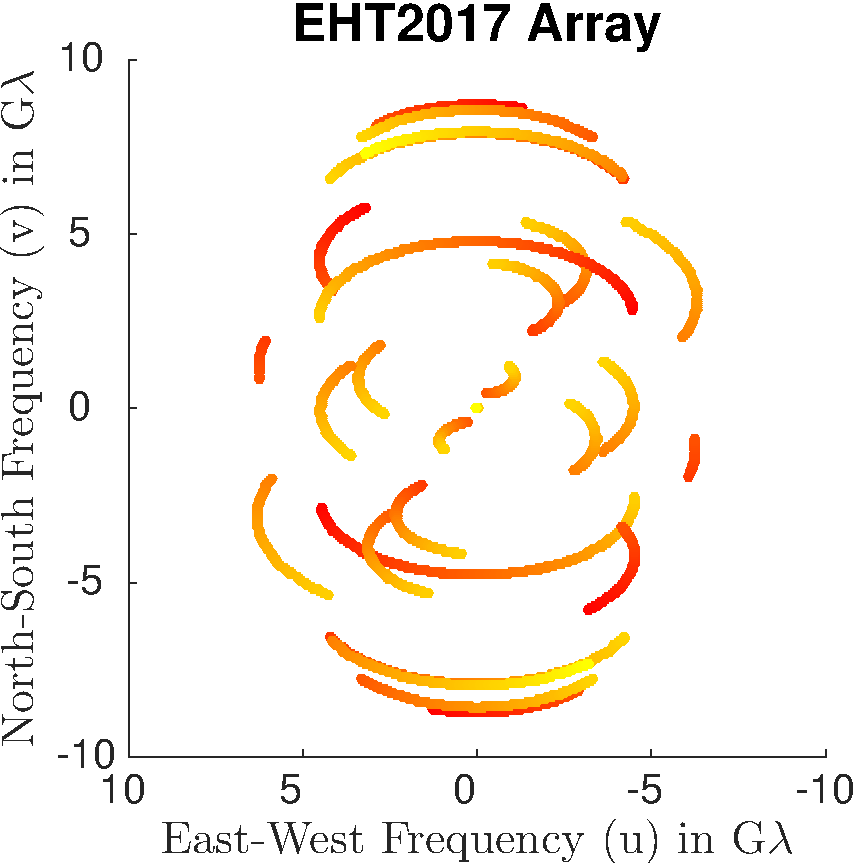
\includegraphics[trim=0cm 0 0 -4cm,height=.43\linewidth]{figures/uvcoverage/uv_eht2017_2.pdf}}
			 		\qquad  }}
			 &  \hspace{-0.7cm}  \large{\textsf{Truth}}   & &  \large{\textsf{a = 2}} & \large{\textsf{a = 5}}  &  \large{\textsf{a = 10}}    \\
			&  \hspace{-0.5cm} {{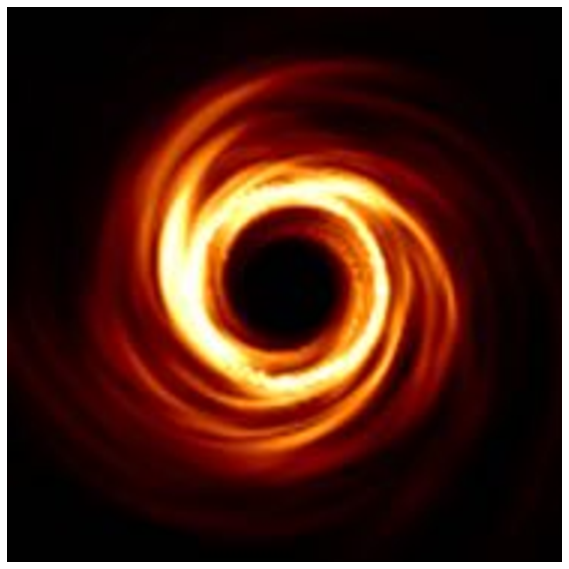
\includegraphics[height=.13\linewidth]{figures/singleimage/visibilities/hotakaframe3.pdf}} } &
			\multirow{1}{*}[0.82in]{ \rotatebox[origin=t]{90}{ \small{\textsf{Gauss. Recon.}} }}
			&
			{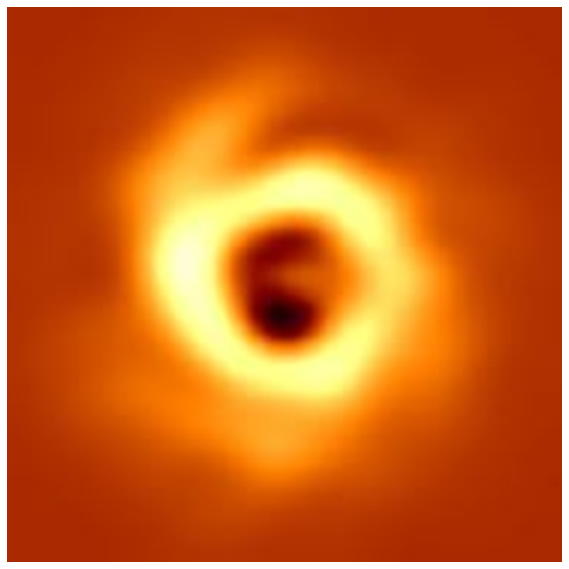
\includegraphics[height=.13\linewidth]{figures/singleimage/visibilities/img_powerdropoff_2.pdf}} &
			{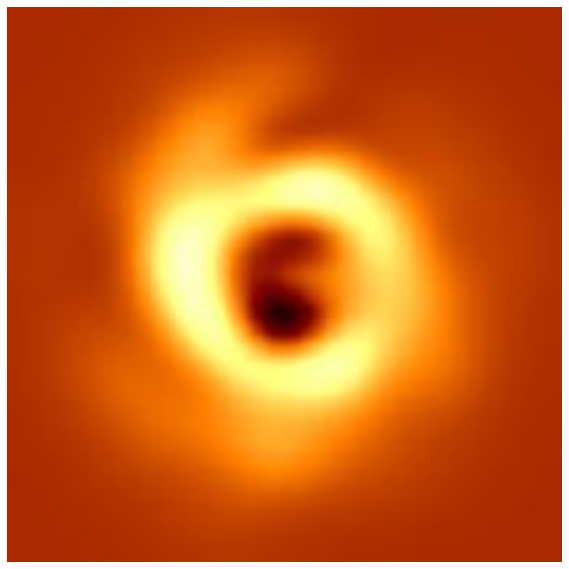
\includegraphics[height=.13\linewidth]{figures/singleimage/visibilities/img_powerdropoff_5.pdf}} 
			&
			{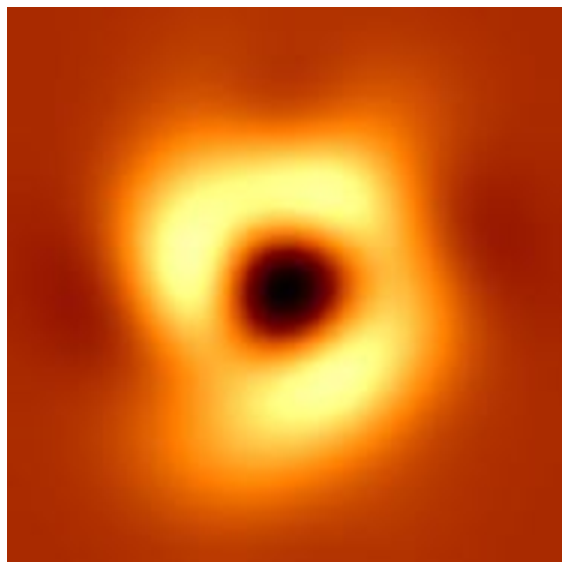
\includegraphics[height=.13\linewidth]{figures/singleimage/visibilities/img_powerdropoff_10.pdf}} 
			\\
			& \vspace{-.0in}  \hspace{-0.8cm} \large{\textsf{MEM \& TV}}  & &  \multicolumn{3}{c}{ 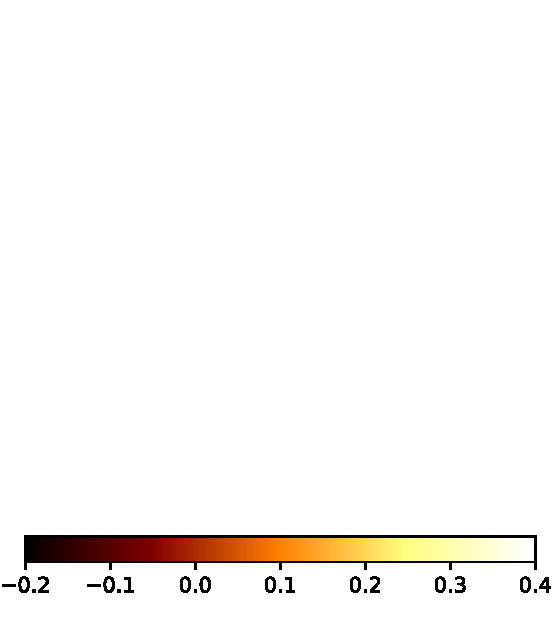
\includegraphics[width=.25\linewidth]{figures/cbar/horizontal_cbar_-2to4_r2.pdf} }
			\\
			%& \vspace{-.15in}  \hspace{-0.8cm} \large{\textsf{MEM \& TV}}  & & & &       \\
			&\hspace{-0.5cm} {{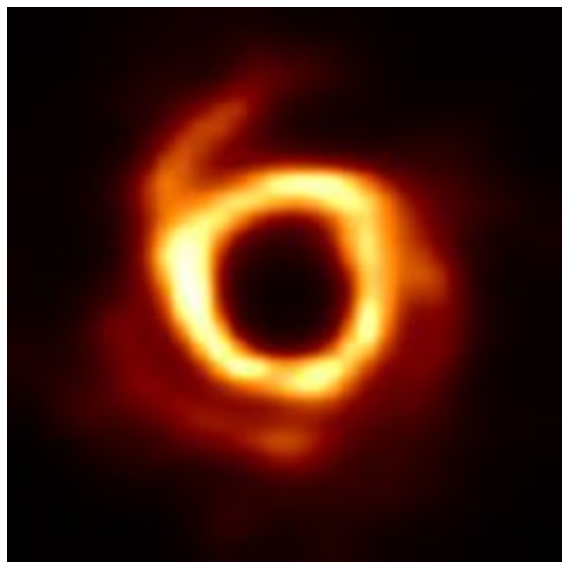
\includegraphics[height=.13\linewidth]{figures/singleimage/visibilities/img_maxen.pdf}} } &
			\multirow{1}{*}[0.82in]{ \rotatebox[origin=t]{90}{ \small{\textsf{Clipped Recon.}} }}
			&
			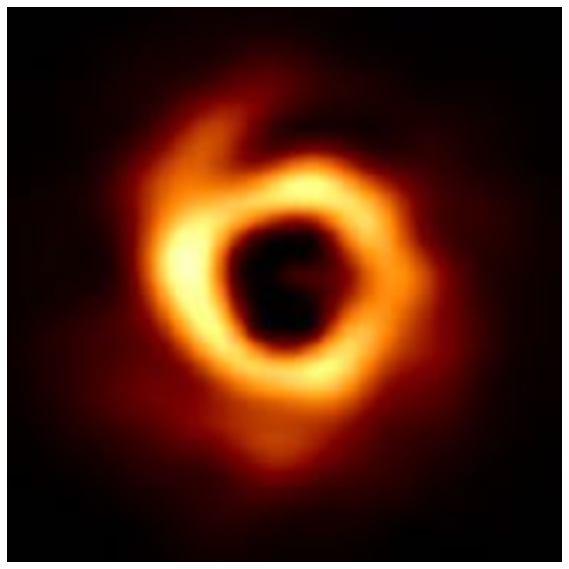
\includegraphics[height=.13\linewidth]{figures/singleimage/visibilities/imgClip_powerdropoff_2.pdf} &
			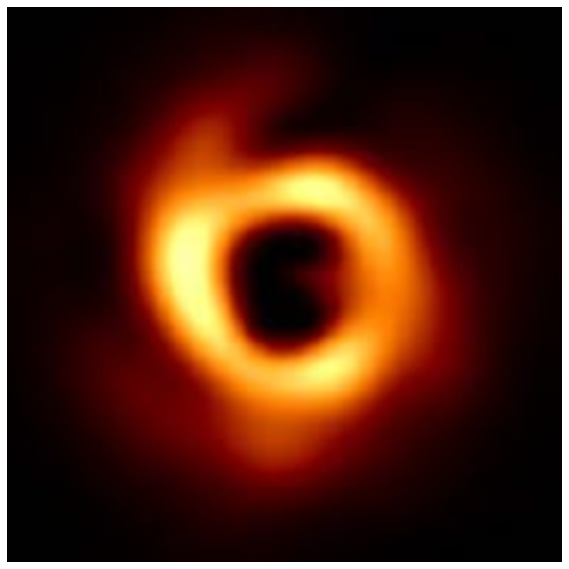
\includegraphics[height=.13\linewidth]{figures/singleimage/visibilities/imgClip_powerdropoff_5.pdf} &
			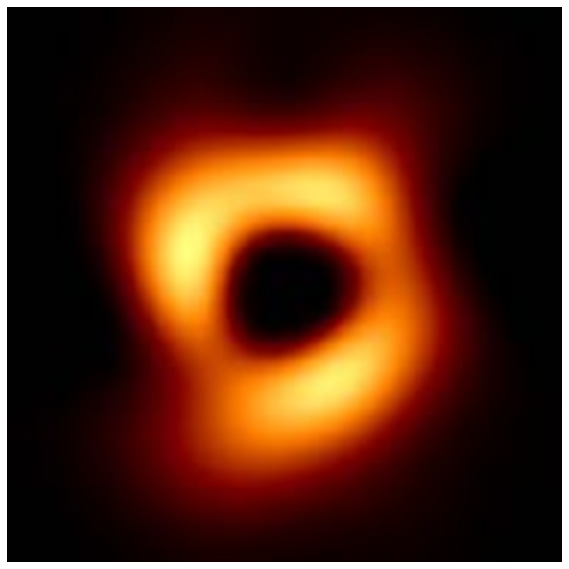
\includegraphics[height=.13\linewidth]{figures/singleimage/visibilities/imgClip_powerdropoff_10.pdf} 
			\\
			& \vspace{-.0in} \hspace{-.8cm} \large{\textsf{CHIRP}}  & &  \multicolumn{3}{c}{ 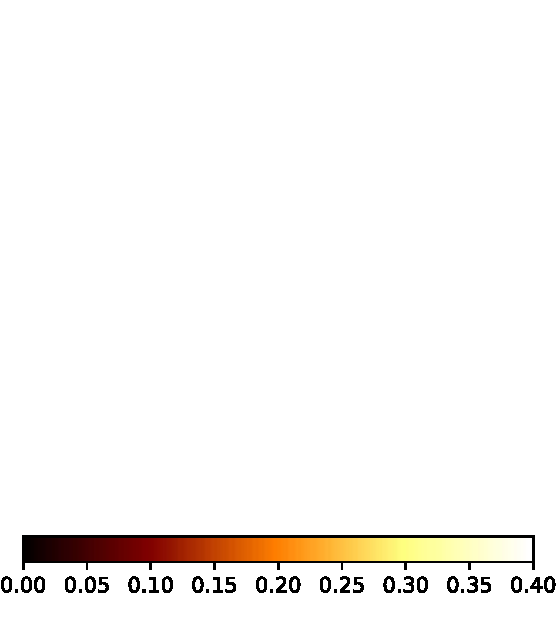
\includegraphics[width=.25\linewidth]{figures/cbar/horizontal_cbar_0to4_r2.pdf} }
			\\ 
			%& \vspace{-.15in} \hspace{-.8cm} \large{\textsf{CHIRP}}   & & & &     \\
			&\hspace{-0.5cm} {{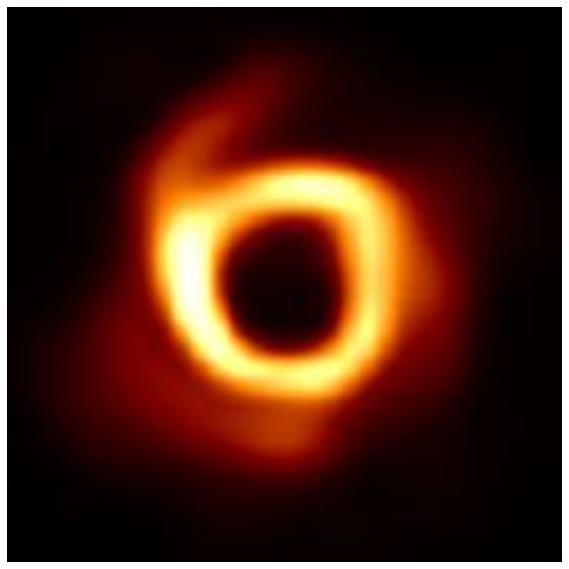
\includegraphics[width=.13\linewidth,trim=0.0cm -1.5cm 0.0cm 0.0cm]{figures/singleimage/visibilities/hotakaframe_chirp.pdf}} \vspace{0.04cm} } &
			\multirow{1}{*}[1.05in]{ \rotatebox[origin=t]{90}{ \small{\textsf{Diagonal Std. Dev. }} }}
			&
			\hspace{-.1in} 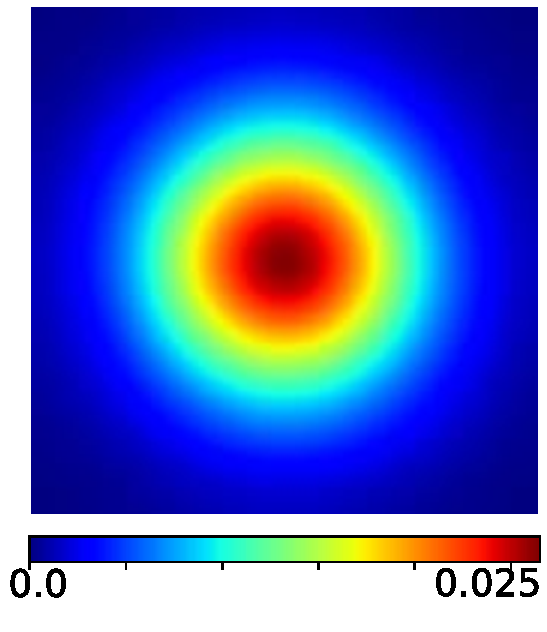
\includegraphics[width=.138\linewidth]{figures/singleimage/visibilities/covImg_powerdropoff_2_r2.pdf} &
			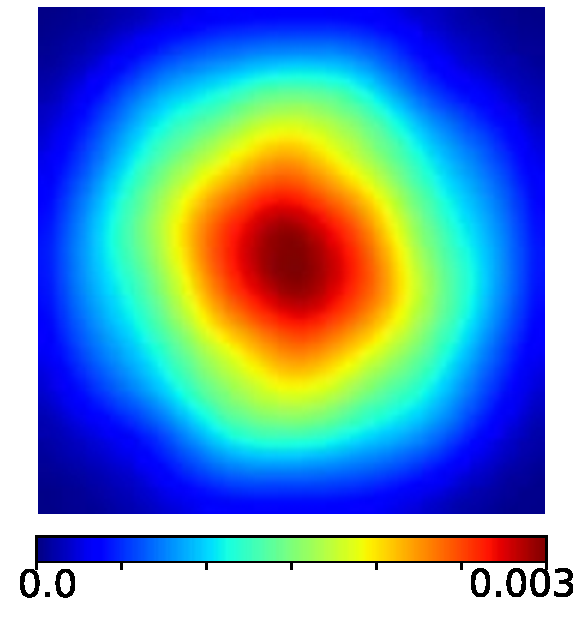
\includegraphics[width=.148\linewidth]{figures/singleimage/visibilities/covImg_powerdropoff_5_r2.pdf} 
			&\hspace{-.1in}
			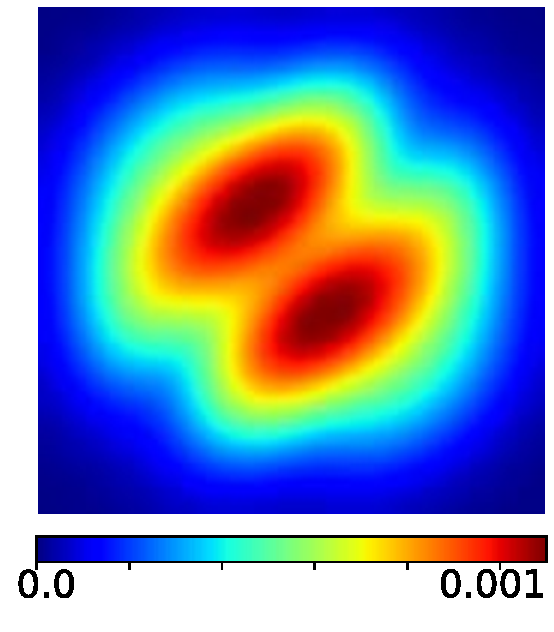
\includegraphics[height=.145\linewidth]{figures/singleimage/visibilities/covImg_powerdropoff_10_r2.pdf} 
		\end{tabular}
		\caption{{\bf Static Imaging Comparison:} Results of static imaging using a multivariate Gaussian prior ( \textsf{a} = 2, 5, 10) compared to state-of-the-art reconstruction methods using MEM \& TV regularizers~\cite{andrew} as well as patch-based regularizers (CHIRP)~\cite{bouman2016computational}. All images are shown with a field of view of 160 $\mu$-arcseconds. Data is generated using a static image with the uv-coverage of the EHT2017 array shown on the left (see Section~\ref{sec:results}). The uv-coverage is colored by time, as indicated by the colorbar in Figure~\ref{fig:uvcov2}. Note however that in this static imaging case the time of measurements is not relevant. Although the previous algorithms (MEM \& TV and CHIRP) both produce better results, the Gaussian reconstruction is able to correctly get the broad structure of the underlying image. Since we do not impose positivity, negative values are reconstructed. However, by clipping the resulting image we can see that the result aligns well with the true static image. The Gaussian prior model also allows us to easily estimate our reconstructed image uncertainty. We visualize the diagonal entries of the posterior covariance matrix as the reshaped standard deviation image. Note that as the smoothness parameter \textsf{a} is increased, the per-pixel standard deviation becomes smaller, but the structure of the standard deviation deviates from what was specified in the prior (recall $\bLambda$ is scaled by $\bmu$, which we have specified as a 2D Gaussian in this work). For large \textsf{a} the uncertainty is shown to be primarily in the diagonal north-west to south-east direction, due to the lack of spatial frequencies sampled by the telescope array in this direction. To avoid approximations and best show the recovered posterior covariance matrices, atmospheric error has not been included in the data used to recover these images. The scaling of the colormaps is in mili-Jansky per squared $\mu$-arcsecond. } 
		\label{fig:staticimaging}
		%-.2, .4
		%0, .4
	\end{center}
	\vspace{-.2in}
\end{figure*}



\vspace{-.2in}
\subsection{Multivariate Gaussian Image Prior}
\label{sec:gauss_prior}

A prior distribution on $\im$ constrains the space of possible solutions during inference, and can be defined in a variety of ways.
%There are many ways that a prior distribution on $\im$ can be defined. 
For instance, maximum entropy, sparsity, and patch priors have been all used previously for VLBI imaging~\cite{andrew,kazu,bouman2016computational, rusenimaging}.
%Priors that have been used previously in VLBI imaging include maximum entropy, sparsity, and patch priors. 
In this work we instead choose to define the underlying image, $\im$, as being a sample from the distribution $\mathcal{N}_{\im}(\bmu, \bLambda)$. This choice leads to less sharp image reconstructions compared to richer priors, %is less powerful 
%expressive
%than some of the other image priors in reconstructing a sharp image, 
%but its simple expression 
%comes with the advantage of allowing 
%allows for a better theoretical understanding of our solutions, which proves especially valuable when propagating uncertainties in dynamical imaging (refer to Section~\ref{sec:dynamic_inference}). 
but its simplicity allows for a cleaner understanding of our solutions. This proves especially valuable in propagating uncertainties during dynamic imaging (refer to Section~\ref{sec:dynamic_inference}). 
%is less expressive
%allows for a better theoretical understanding of our solutions that BLAH BLAH BLAH.  

%Image regularizers that enforce spatial smoothness can often be described with a multivariate Gaussian image prior. 
%For instance, the common squared total variation regularizer can be expressed by writing the image covariance, $\bLambda$, in terms of  the $ 2 \npix^4 \times \npix^4$ gradient matrix, $\bm{G}$: $\bLambda \propto \left[ \bm{G}^T \bm{G} \right]^{-1}$.

Studies have shown that the average power spectrum of an image often falls with the inverse of spatial frequency in the form $1/(u^2 + v^2)^{a/2}$, where $a$ is a value that specifies the smoothness of the image~\cite{torralba2003statistics}. 
%$1/f^a$. %(Burton and Moorhead 1987, Field 1987, 1994, Tolhurst et al 1992) http://web.mit.edu/torralba/www/ne3302.pdf
As the amplitude of a spatial frequency is linearly related to the image itself, this statistical property can also be enforced by specifying the covariance in a prior distribution. Specifically, 
%\begin{align}
%\bLambda'  =  &  \bm{W}^{*T}  \mbox{diag} \left[ \frac{1}{ %(\bm{u}^2 + \bm{v}^2)^{a/2} } \right]  \bm{W} 
%\end{align}
\begin{align}
& \hspace{.5in} \bLambda'  =    \bm{W}^{*T}  \mbox{diag} \left[ \bm{b}  \right]  \bm{W}  \\ 
b[i] = & \begin{cases} 
({u[i]}^2 + {v[i]}^2)^{-a/2}  & {u[i]}^2 + {v[i]}^2 > 0 \\
\epsilon & {u[i]}^2 + {v[i]}^2  = 0 \\
\end{cases}
\end{align}
\noindent{for DFT matrix $\bm{W}$ of size $M^2 \times M^2$ %and vector $\bm{b}$ of size $M^2$ 
for an $M\times M$ pixel image and a small positive value, $\epsilon$. Each row of $\bm{W}$ and $\bm{b}$ %is comprised of $\vecFTmtx(u,v)$ (see Section BLAH), and 
	corresponds to a $(u,v)$ coordinate in the 2D grid of frequencies, \{ $S \times S$ \}, for }
\begin{align}
%UV &= S \times S = \{ (u,v) | u \in S, v \in S \} \\
S &= \left\{ \frac{m-M/2}{FOV} \right\}, m\in \mathbb{Z}: m \in [0,M-1],
\end{align}
where $FOV$ is the image's field of view in radians.
To specify the variance of each pixel and help encourage positivity, we modify the amplitude of the covariance by left and right multiplying by ${c \cdot \mbox{diag}[\bmu ]} $:
\begin{align}
\bLambda = c^2 \mbox{diag}[\bmu ]^T \bLambda' \hspace{0.01in} \mbox{diag}[\bmu ] 
\end{align}
\noindent{A $c$ value of 1/3 implies that 99\% of flux values sampled from $\mathcal{N}_x(\bmu, \bLambda)$ will be positive. In this work we have chosen $\mu$ to be a circular Gaussian with a standard deviation of 40-50\% of the reconstructed FOV to encourage most of the flux to stay near the center of the image and away from the edges. Figure~\ref{fig:priorsamples} shows the covariance matrix constructed for $a=2,3,4$ along with images sampled from the prior  $\mathcal{N}_x(\bmu, \bLambda)$. Notice that as $a$ increases, the sampled images are smoother. Thus, $a$ provides the ability to tune the desired smoothness of the inferred images. 
}

%THIS DOESNT BELONG HERE!!!
%In Section BLAH we explain how this image prior can be introduced into the estimation of each $x_t$. Introducing the prior into the estimate of each image helps to further constrain the images in this very ill-posed setting. 


\subsection{Inference}
\label{sec:static_inf}

%As a Gaussian distribution is a conjugate prior for a Gaussian likelihood, the posterior distribution 

Our goal is to find the most likely image, $\im$, that describes the data products we have observed, $\meas$. A maximum a posteriori (MAP) solution is found by maximizing the log-posterior from Equation~\ref{eq:bayes}:
\begin{align}
\hat{\im}  = \argmax_{\im} & \log p(\im|\meas) \\
\notag =  \argmin_{\im}  &\left[ (f(\im)-\meas)^T \bR^{-1} (f(\im)-\meas) \right. \\
& \left. + (\im-\bmu)^T \bLambda^{-1} (\im-\bmu) \right] .
\end{align}

Note the similarities of this equation's structure to that of previous static imaging methods in Equation~\ref{eq:setup} and~\ref{eq:chi2}. 
Although the hyperparameter $\gamma$ is no longer explicit, the scaling of $\bLambda$ acts like this hyperparameter and balances influence of the measured data with influence of the prior.
%used in many VLBI imaging frameworks.

%\subsection{Data Likelihood - change from likelihood}


\vspace{0.1in}
\subsubsection{Linear Measurements}


As explained in Section~\ref{sec:dataproducts}, $f(\im)$ is linear when $\meas$ is composed solely of calibrated complex visibilities with no %remaining
atmospheric error.
In this case -- when $f(\im) = \FTmtx \im$ --
%with corresponding Gaussian noise of variance, $\bm{\sigma}^2$  (i.e. no atmospheric error), 
a closed-form solution of $\hat{\im}$ can be found %. 
%In the case that $f(\im) = \FTmtx \im$ is a linear function of $\im$,a closed-form solution of $\hat{x}$ can be found. 
%In this situation, $\im$ can be solved 
through traditional Weiner filtering. Specifically, we can compute the most likely estimate of each $\im$ as: 
% Equation~\ref{eq:map}:
\begin{align}
\hat{\im} &=  \bmu  + \bLambda {\bf F}^T ( \bR + \FTmtx \bLambda \FTmtx^{T} )^{-1} (  \meas -  \FTmtx \bmu ) .
\label{eq:map}
\end{align}
\noindent{
	%Refer to the supplemental material for details of this derivation. 
	In the limit of having no prior information about the underlying image $\im$, e.g.,  $\bLambda = \lim_{\lambda \to\infty} \lambda \mathds{1}$ for identity matrix $\mathds{1}$, this MAP solution reduces to $\hat{\im} =  \FTmtx^{+} \meas$. In other words, in the absence of prior image assumptions, the noise on each measurement, $\bR$, is no longer relevant and the reconstructed image is simply obtained by inverting $\meas = \FTmtx \im$.
	This is very similar to reconstructing the ``dirty image''~\cite{taylor1999synthesis}.
	
%When $\meas$ are sparse visibilities, although $\FTmtx^{-1}$ is undefined, since $\FTmtx \FTmtx^{*T} = \mathds{1}$, $\hat{\im} =  \FTmtx^{-1} \meas$ is very similar to reconstructing the ``dirty image''~\cite{taylor1999synthesis}.

%evaluating, inspecting

The same solution can also be obtained by evaluating %and inspecting 
the posterior distribution. 
With a linear measurement function, $f(\im)$, the proposed Gaussian formulation leads to a closed-form expression for the posterior. In particular, 
\begin{align}
p(\im|\meas) & = \mathcal{N}_{\im} (\hat{\im}, \bm{C} ). 
\end{align}
for covariance matrix
%\noindent{The mean of this posterior distribution is equivalent to the MAP estimate obtained through Weiner Filtering.}
%Our proposed Gaussian formulation not only facilitates easily computing the MAP estimate, but also the uncertainty in the estimated $\hat{\im}$:
\begin{align}
\bm{C} = \bLambda - \bLambda \FTmtx^T ( \bR + \FTmtx \bLambda \FTmtx^T )^{-1} \FTmtx \bLambda .
\end{align}
\noindent Estimating uncertainty with the covariance matrix is useful in understanding what regions of the reconstructed image we trust. This becomes especially helpful when propagating information in dynamical imaging, as will be demonstrated in Figure~\ref{fig:propinfo}. 




\vspace{0.1in}
\subsubsection{Non-linear Measurements}
%When the data products in $\meas$ are invariant to atmospheric noise, $f(\im)$ is a non-linear function of $\im$ and a closed-form solution does not exist. 
When $f(\im)$ is a non-linear function of $\im$, as is the case when the data products in $\meas$ are invariant to atmospheric noise, a closed-form solution does not exist. 
%of atmospheric noise, large phase errors are added to the complex visibility measurements. However, these phase errors are incorporated in a way that preserves closure phase (refer to Section BLAH). In order to handle this additional phase error, without having to explicitly model the errors as latent variables, we can change the measurement function, $f(.)$, to one that is invariant to atmospheric inhomogeneity.
%A measurement function, $f(.)$, which extracts the bispectrum, visibility amplitude, or closure phase would be invariant to this atmospheric inhomogeneity. However, it comes at the expense of being a non-linear function of the image, $x$. 
However, to solve for the optimal $\im$ we linearize $f(\im)$ to obtain an approximate solution, $\hat{\im}$. Using a first order Taylor series expansion approximation around $\tilde{\im}$, we approximate the data likelihood as
\begin{align}
p(\meas|\im) = \mathcal{N}_{\meas}(f(\im),\bR) \approx \mathcal{N}_{\meas} \left( f( \tilde{\im} ) +  \dot{\FTmtx} (\im - \tilde{\im} )  , \bR \right) , 
\end{align}
\noindent{ for $\dot{\FTmtx} = \left. \frac{df(\im)}{d \im} \right| _{\tilde{\im} }$. Using this approximation, % we solve for 
	the optimal $\hat{\im}$ is}
\begin{align}
\hat{\im} &=  \bmu  + \bLambda \dot{\FTmtx}^T ( \bR + \dot{\FTmtx} \bLambda \dot{\FTmtx}^{T} )^{-1} (  y  - f(\tilde{\im}) +  \dot{\FTmtx} (\tilde{\im}-\bmu) ) .
\label{eq:approxoptimal}
\end{align}

To further improve the solution, we solve Equation~\ref{eq:approxoptimal} iteratively by updating  $\hat{\im}$ and setting $\tilde{\im} = \hat{\im} $ until convergence.
%By iteratively solving for Equation~\ref{eq:approxoptimal} and setting $\tilde{\im} = \hat{\im} $, we can improve our estimated image reconstruction, $\hat{\im}$. 
Note that in the case that $f(\im)$ is linear, $\dot{\FTmtx} = \FTmtx$ and Equation~\ref{eq:approxoptimal} reduces to Equation~\ref{eq:map}. We compare results of this reconstruction method to other state-of-the-art methods for a static source in Figure~\ref{fig:staticimaging}. Figure~\ref{fig:staticimaging} demonstrates that, although this approach does not outperform other state-of-the-art static imaging methods, reasonable results are achieved despite a simpler image regularizer and optimization procedure. This simpler approach will become useful in developing a dynamic imaging approach. 

